\chapter{Lecture 3: Combinatorics} \label{lect3}
We mentioned in example \ref{example2.2.1} that we will soon find a way to count outcomes without listing them all; in this section we will do just that. Combinatorics \label{combinatorics} is a branch of mathematics that involves counting ways in which objects can be chosen, combined, and ordered. We will use results from combinatorics to \label{order2}
\begin{itemize}
\item
Find the sizes of certain sets;
\item
Count the number of occurrences of a particular type of element or subset in a set;
\item
Count the number of ways of selecting (or sampling) certain elements or subsets.
\end{itemize}
The two most important ideas that we will discuss when doing combinatorics will be \textbf{order} and \textbf{replacement}. \label{replacement}
\subsection{Example}
Suppose we have a set of 15 crayons, all of different colours. Now, suppose we want to choose 2 of those crayons and record their colour. We can do this in two ways;
\begin{enumerate}
\item
Choose 1 crayon, write down its colour, then \textbf{put the crayon back} in the set before choosing the second crayon; 
\item
Alternatively, choose 1 crayon, \textbf{set it aside} in a different pile, then choose the second crayon.
\end{enumerate}
How does the choice of method affect the outcome of sampling crayons? Well, for starters, in case 1 we can end up choosing two crayons of the same colour; whereas in case 2 we will only ever end up with 2 different coloured crayons. Case 1 is referred to as \textit{sampling with replacement}, while case 2 is referred to as \textit{sampling without replacement.}

\subsection{Example}
Have another look at the dice examples from
%REFERENCE TO ``LECTURE'' AS A SECTION NAME!!!
lecture 2 (example~\ref{example2.2.1} and example~\ref{example2.2.4}). When defining the outcome space in example \ref{example2.2.1} the \textbf{order} of the dice was important. In example \ref{example2.2.4}, on the other hand, we didn't care which dice had rolled which number, i.e. the order was not important. Notice that not caring about order significantly reduced the size of the outcome space in example \ref{example2.2.4}. For example, when order was disregarded the element $(1,5)$ became equal to the element $(5,1).$

\subsection{Ordered and unordered lists}
A list of objects (or outcomes) in a specific order is called a \textbf{permutation}. Consider the set $\set{1,2,3}$. If we list the numbers 1 to 3 in their natural order we get $1,2,3.$ We could also change this order by listing the numbers in order as $2,3,1$ or as $1,3,2$ for example.  What you have seen is three \textbf{permutations} of the ordered set $\set{1,2,3}$. \label{combination} \label{permutation} \\

\noindent A list of objects in which the order is not considered is called a \textbf{combination}. We could choose to regard the set $\set{1,2,3}$ as a combination. In this case we do not write lists like $1,2,3$ or $2,3,1$ as these are no different from each other, so we simply refer to the unordered set (i.e. the combination) $\set{1,2,3}.$ \\

\noindent This terminology actually conflicts with our everyday use of the word combination. For example, in everyday English we would refer to the digits on a bicycle lock as a combination, and we call the lock itself a combination lock. In mathematical terms this everyday terminology makes no sense. The digits on a bicycle lock have an order to them, and this order is important, so in mathematical terms the digits on a bicycle lock form a permutation. If we get the permutation right, then we release the lock.

\subsection{The multiplication rule} \label{secmult}
We will need to use the term, \textbf{independent trials}, to describe this rule. Note that this term has not yet formally been defined by us; this will be remedied during section \ref{independence} on page \pageref{independence}. Feel free to flip forward and read the introduction to that section to get an intuitive idea of \textbf{independence}. \\

 
\noindent In example \ref{outcome space} we listed the entire outcome space for the experiment of flipping a fair coin then rolling a standard balanced die. This is an experiment with two trials: flip a coin, then roll a die. We can think about this visually as

\begin{center}
	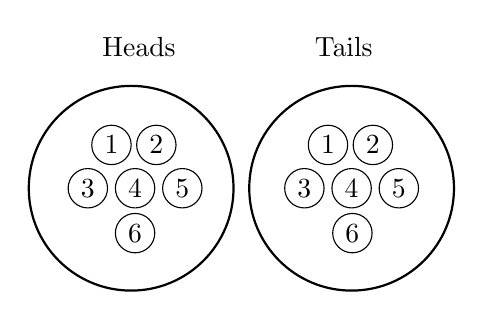
\begin{tikzpicture}
	%\draw [fill = white] (-0.5,0.8) ellipse (1.6cm and 0.8cm);
	\draw [thick, fill = white] (1.4,0) circle (1.3);
	\draw [thick, fill = white] (-1.4,0) circle (1.3);
	%\draw [thick] (1.4,0) circle (1.5);
	%\draw [thick] (-0.5,0.8) ellipse (1.6cm and 0.8cm);
	\draw (1.3,1.8) node {Tails};
	\draw (-1.3,1.8) node {Heads};
	\draw (-1.35,0) circle (0.25) node {$4$};
	\draw (-0.75,0) circle (0.25) node {$5$};
	\draw (-1.95,0) circle (0.25) node {$3$};
	\draw (-1.65,0.55) circle (0.25) node {$1$};
	\draw (-1.08,0.55) circle (0.25) node {$2$};
	\draw (-1.35,-0.57) circle (0.25) node {$6$};
	
	\draw (-1.35+2.75,0) circle (0.25) node {$4$};
	\draw (-0.75+2.75,0) circle (0.25) node {$5$};
	\draw (-1.95+2.75,0) circle (0.25) node {$3$};
	\draw (-1.65+2.75,0.55) circle (0.25) node {$1$};
	\draw (-1.08+2.75,0.55) circle (0.25) node {$2$};
	\draw (-1.35+2.76,-0.57) circle (0.25) node {$6$};
	%\draw (0,0) node {$A \cap B$};
	\end{tikzpicture}
	%\caption{Venn Diagram of $A$ and $A^c.$}
\end{center}

\noindent For the first trial (flip a coin) we have 2 possible outcomes, represented by the larger circles. For the second trial (roll a die) we have 6 possible outcomes, represented by the smaller circles. As we can see from the picture there are a total of $2\times6 = 12$ possible outcomes for the experiment. This is the size of the outcome space $\Omega$ from example \ref{outcome space}. \\

\noindent We now introduce a generalisation of this idea, called the multiplication rule. \\

\noindent \textbf{Multiplication rule:} \\
If a task can be broken up into $\mathbf{k}$ \textbf{independent trials} (or stages), and the first stage can be done in $\mathbf{n_1}$ ways, and the second stage can be done in $\mathbf{n_2}$ ways, and so on, with the last stage doable in $\mathbf{n_k}$ ways. Then the number of ways, $\mathbf{N}$, of doing the whole task is
\[
N = n_1\times n_2 \times \ldots \times n_k
\]
\subsection{Example} \label{ex3.0.9}
In example \ref{example2.2.1} we have 2 independent trials; roll the first die, then roll the second die. So~$k~=~2$. On each of the two trials there are 6 possible outcomes (roll a number 1 to 6). So $n_1 = 6$ and $n_2 = 6$. We want to know the size, $N$, of the outcome space. Using the multiplication rule we get
\[
N = n_1 \times n_2 = 6 \times 6 = 36.
\]
So, as we claimed in example \ref{example2.2.1}, the outcome space has a size of 36. \\

\noindent Why don't we use the same method for example \ref{example2.2.4}? The answer is that the number, $k$, of independent trials in example \ref{example2.2.4} is only 1. In \ref{example2.2.4} we disregard order. So, instead of, ``rolling one die then rolling the other die'' we just have 1 trial, ``roll both of the dice.''

\subsection{Example} \label{example1}
Suppose that 5 Australian birds attempt to fly over the Pacific Ocean (the largest ocean on earth), to try and reach America. Soon, they get very tired and decide to find somewhere to land. They spot 7 floating objects. How many different ways can the birds arrange themselves if each bird gets one floating object? That is, how many different permutations of the birds can we have if the birds are ordered by their choice of object? Well, we have 5 birds to land, so we have 5 independent trials. The first bird has 7 choices for places to land, so $n_1 = 7$. The second bird has 6 choices (the first bird already took one of the floating objects), so $n_2 = 6$, the third bird has 5 choices, so $n_3 = 5$, and so on. Using the multiplication rule, the number of permutations $N$ is thus
\[
N = n_1\times n_2 \times n_3 \times n_4 \times n_5 = 7\times 6 \times 5 \times 4 \times 3 = 2520.
\]
So there are 2520 different possible permutations of the birds!

\subsection{Example} \label{example2} \label{80books}
I have 80 books on my book shelf. How many different ways can I arrange these books? \\

\noindent Let's start by taking all of the books off of the bookshelf, then picking up the books one at a time and putting them back on the shelf. I will do this for all 80 books, so $k = 80$. When I pick up the first book there are 80 to choose from so $n_1 = 80$. Choosing the second book I have 79 choices so $n_2 = 79$. This pattern continues until I get to the last book with $n_{80} = 1$. I want to find the number $N$ of possible orderings that I could have chosen the books in (the number of permutations). Using the multiplication rule I get
\[
N = 80\times79\times78\times\ldots\times 3\times2 \times1. \label{example3}
\]
This is quite a large number. It is too big to bother writing here. It is not \textit{ridiculously} large; there are bigger numbers. It is however, a number much greater than the estimated total number of \textit{atoms in the known universe}. It is remarkable that there are supposedly more ways of arranging 80 books on my bookshelf than there are atoms in the known universe. For information on a truly ridiculous number however, search youtube for the \textit{numberphile} video on \textit{Grahams number}. 

\subsection{Factorial notation}
The number $80\times79\times78\times\ldots\times 3\times2 \times1$ from example \ref{example3} above is best expressed using factorial notation; that is, we write $80!.$ The factorial symbol looks similar to an exclamation mark, but its meaning is different. For any number $n$, we write \label{!} \label{factorial}
\[
n! = n\times (n-1) \times (n-2) \times \ldots \times 3 \times 2 \times 1.
\]
So, for example, the number 5! is
\[
5! = 5\times 4 \times 3 \times 2 \times 1 = 120.
\]
Finally, a very important definition in factorial notation is
\[
0! = 1.
\]
This means, for example, that if we divide by $0!$ we are \textit{not} dividing by zero; we are dividing by 1. So
\[
\frac{1}{0!} = \frac{1}{1} = 1
\]


\subsection{Selection (sampling) with/without order and with/without replacement} \label{ordered sampling}
Notice that in the last two examples (examples \ref{example1} and \ref{example2}) we made ordered choices out of a pool of things (a pile of books or a collection of floating objects) where each choice that we made reduced the number of available things. This scenario is referred to as \textbf{ordered sampling without replacement}. Whenever we make $r$ choices out of a pool of $n$ things, there are several possibilities, \label{sampling}
\begin{itemize}
\item
Previous choices have no effect on the pool of available choices, and order is considered \\ (\textbf{ordered sampling with replacement});
\item
After a choice is made, any later choice has to be different \\ (\textbf{ordered sampling without replacement});
\item
Every choice has to be different, but there is no sense of order \\ (\textbf{unordered sampling without replacement}).
\end{itemize}
Notice that we have omitted a fourth case, the case of unordered sampling with replacement. This was intentional, as this case is a little more complicated than the other cases (and it is not covered in this course). If you are still interested, have a look at the open access peer-reviewed online component of Introduction to Probability, Statistics, and Random Processes by Hossein Pishro-Nik. Searching online for ``probability course 2.1.4 unordered sampling with replacement'' should return the correct result.

\subsection{Example}
A couple of Jedi, Luke and Obi-Wan, decide to head to the imperial pound and free some Wookiees. 
Which combination of sampling with/without order and with/without replacement applies to each of the following tasks?
\begin{enumerate}
\item
Luke decides which Wookiee he wants to rescue first, then Obi-Wan decides which Wookiee he wants to rescue (they may or may not pick the same Wookiee).
\item
Two of the Wookiees wander over and become separated from the rest. Luke and Obi-Wan decide to save those two.
\item
Luke runs in and saves a Wookiee, then Obi-Wan runs in and saves a second Wookiee.
\end{enumerate}
Solution: (1) \textit{Ordered sampling with replacement.} (2) \textit{Unordered sampling without replacement.} (3) \textit{Ordered sampling without replacement.}

\section{Counting possible choices}
\subsection{Ordered sampling with replacement}
This is the simplest of the three cases. It is essentially an application of the multiplication rule. Suppose we want to choose $r$ things from a pool of $n$ things. For the first choice we have $n$ different possible choices, so $n_1 = n$. For the second choice we have, again, $n$ difference possible choices, so $n_2 = n$. For every one of our $r$ choices we have $n$ possible things to choose from, since this is sampling \textit{with} replacement. We want the number, $N$, of total possible choices. Using the multiplication rule
\[
N = n_1 \times n_2 \times \ldots \times n_r = \underbrace{n \times n \times \ldots \times n}_{\text{$r$ times}} = n^r.
\]

\subsection{Ordered sampling without replacement}
In examples \ref{example1} and \ref{example2} we used the multiplication rule to count choices for ordered sampling without replacement. Here we are going to develop a neat expression for the number of choices, using factorial notation. \\

\noindent Whenever we do ordered sampling without replacement we have a number of trials, and the number of choices decreases as we move through the trials. We make one choice on each trial, so on each trial the number of available choices decreases by 1. We always start with the maximum number of choices available. Suppose that we wish to choose $r$ things from a pool of $n$ things. Then on the first trial we have $n$ available choices, on the second trial we have $(n-1)$ choices, on the third trial $(n-2)$, and so on, and on the final trial we have $(n-r+1)$ choices. Why are we subtracting $r$ then adding $1$ on the final trial? This extra $1$ represents the final trial itself, once this trial is complete and we have zero trials remaining, there would be $n-r$ choices left (we can't use these choices because we have zero trials left, but this is how many choices would remain); it should be clear that taking $r$ things from $n$ things leaves $n-r$ things behind when we are done (and we are done when there are zero trials left). Finally, using the multiplication rule this means that the total number of possible choices, N, is
\[
N = n \times (n-1) \times (n-2) \times \ldots \times (n - r + 2) \times (n - r + 1)
\]

\noindent We can find a neater expression than this, but first let's look at a concrete example. In example \ref{example1} we wanted to make $5$ choices from a pool of $7$ things. So $n = 7$, and $r = 5$. So we want there to be $2$ choices left when we have zero trials remaining, or in other words  $n - r = 7 - 5 = 2$ (again, we can't \textit{use} these choices, they are just left over after we have taken our $r$ choices away). This means that on our final (non-zero) trial we want to have 3 choices remaining, in other words $(n - r + 1) = (7-5+1) = 3$. In example \ref{example1} we found the expression
\[
N = 7\times 6 \times 5 \times 4 \times 3.
\]
Have a look at the number 7! (i.e. 7 factorial),
\[
7! = 7\times 6 \times 5 \times 4 \times 3\times 2 \times 1
\]
If we divide by 2! we get
\[
\frac{7!}{2!} = \frac{7\times 6 \times 5 \times 4 \times 3\times 2 \times 1}{2\times 1} = 7\times 6 \times 5 \times 4 \times 3 = N
\]
In the explanation above we found that $(n-r) = 2$. So dividing $n!$ by $(n - r)!$ (that is, dividing 7! by 2!) has just given us the correct expression for $N$; but will this always work when we are doing ordered sampling without replacement? The answer is yes, but let's see why. Our goal is to prove to ourselves that
\[
\frac{n!}{(n-r)!} = \boldsymbol{n(n-1)(n-2)\ldots(n-r+2)(n-r+1)}
\]
Well, let's expand out the expression on the left hand side of the equality,
\[
\frac{n!}{(n-r)!} = \frac{\boldsymbol{n(n-1)(n-2)\ldots(n-r+2)(n-r+1)}\times(n-r)\times(n-r-1)\times\ldots\times2\times1}{(n-r)\times(n-r-1)\times\ldots\times2\times1}
\]
Notice that the terms $(n-r)\times(n-r-1)\times\ldots\times2\times1$ all cancel. So we are left with 
\[
\frac{n!}{(n-r)!} =  \boldsymbol{n(n-1)(n-2)\ldots(n-r+2)(n-r+1)}, \qquad \text{as required.}
\]
So finally we have our neat expression
\[
N = \frac{n!}{(n-r)!}. \label{nPr}
\]
This expression is so commonly used that it has a separate notation. We write $^nP_r$ where the $P$ stands for permutations. Sometimes it is written $nPr$ or even $P(n,r)$.

\subsection{Unordered sampling without replacement} \label{sec313}
We are going to find (and make good use of) a neat expression for counting possible choices when the process of choosing is unordered sampling without replacement. We will use our formula for $^nP_r$ from the previous section to help us derive this expression. \\

\noindent Consider the difference between ordered sampling without replacement and unordered sampling without replacement; the only difference is in the lack of order in the sample. In other words, suppose I want to choose subsets of $3$ numbers from the set $\set{1,2,3,4,5},$ and suppose one of the choices I make is the set $\set{2,3,4}$. If I was doing ordered sampling I might think about the collection $(3,2,4)$ and the collection $(4,3,2)$ as having different orders and thus being different possible choices. Since in unordered sampling these collections are no different from each other, I know that I must have less than (or at most equal to) the number of possible choices that I have for ordered sampling. If we could figure out exactly how many less choices I have, then we could use our formula for $^nP_r$ to derive a formula for the case of unordered sampling. \\

\noindent The key fact to recognise is that for unordered sampling every \textit{permutation} of the set $\set{2,3,4}$ is considered equivalent. To find every permutation, $P$, of an $r$ element set we can use our $^nP_r$ formula, with $n = r$ (ordered sampling of $r$ things from a pool of $r$ things). The formula then simplifies to 
\[
P = \; ^rP_r \; = \frac{r!}{(r-r)!} = \frac{r!}{0!} = r!.
\]
So using $r = 3$ we find there are $3!$ permutations of the set $\set{2,3,4}.$ \\

\noindent So in general, for each \textit{distinct unordered choice} of $r$ things that we can make from a pool of $n$ things, the case of ordered sampling is going to count an extra $r!$ choices that we would prefer to perceive as equivalent to each other. So if we have $N$ \textit{distinct unordered choices}, then $^nP_r$ is going to count an extra $N \times r!$ choices. Thus
\[
^nP_r = Nr!
\]
Rearranging to solve for $N$ (i.e. dividing both sides by $r!$) gives us the formula we want. That is, the number, $N$, of possible unordered choices that we can make is
\[
N = \frac{^nP_r}{r!} = \frac{n!}{r!(n-r)!}.
\]
This formula also has its own (very common) notation. It is sometimes written $^nC_r$ where $C$ stands for ``combination'' (though it is often read ``$n$ choose $r$''). More commonly however, it is written $\binom{n}{r}$, so that
\[
\binom{n}{r} = \frac{n!}{r!(n-r)!}. \label{nCr}
\]
The values that $\binom{n}{r}$ can take are sometimes referred to as the \textbf{binomial coefficients.} We will look at why they are called binomial coefficients in section \ref{secbinom}.

\subsection{Finding probabilities by counting} \label{secprobcounting}
\noindent Recall from section \ref{sec222} (Equally likley outcomes) that, if all of the outcomes $\omega \in \Omega$ are equally likely, then the probability of an event $E$ is given by
\[
P(E) = \frac{|E|}{|\Omega|}.
\]
If $E$ is specified in terms of outcomes, then we can write this as
\[
P(E) = \frac{\text{Number of outcomes in $E$}}{\text{Number of possible outcomes}}.
\]
The next example should illustrate how we can use this.

\subsection{Example}
\noindent A social networking company has recently developed advertising software that matches the behaviour of consumers to a database of 100 typical personality traits. A ranking system is used to decide which 6 personality traits best fit each consumer. The 100 traits were chosen so that any given consumer could be a best match for any of the 100 traits with equal probability. \\

\noindent \textbf{Question 1:} What is the probability that two randomly selected consumers share the same 6 traits? \\
\noindent \textit{Solution:} \\
Let $N$ denote the number of possible outcomes. In this case the number of possible outcomes is equal to the number of possible types of consumer that can be modelled, i.e., the number of possible unique choices of $6$ traits from a pool of $100$, where the order of the traits is not important, which is given by 
\[
N = \binom{100}{6} \tag{unordered sampling without replacement}
\]
We are randomly selecting two consumers. Let $E$ denote the event that the two chosen consumers have the same 6 traits. For our purposes it (perhaps counterintuitively) does not matter what 6 traits the first consumer has, we only care if the second consumer has the same 6 traits as the first. So we are really trying to find the probability that 1 single predetermined type of consumer will be selected from the set of all possible consumer types, $N$. Hence
\begin{align*}
P(E) = \frac{\text{Number of outcomes in $E$}}{\text{Number of possible outcomes}} = \frac{1}{N} & = \frac{1}{\binom{100}{6}}
\end{align*}

\noindent \textbf{Question 2:} 12 of the personality traits were identified as useful by a particular advertising agency; the rest were deemed undesirable. What is the probability that a randomly selected consumer did not have any of the 12 useful traits? \\

\noindent \textit{Solution:} \\
We already know from question 1 that there are $\binom{100}{6}$ possible consumer types. If we remove the 12 useful traits from the pool of 100 traits then we are left with $100 - 12 = 88$ undesirable traits. The number of possible consumers having some set of 6 from these 88 traits is thus
\[
\binom{88}{6}
\]
Let $F$ be the event that a chosen consumer is undesirable. Then
\[
P(F) = \frac{\text{Number of outcomes in $E$}}{\text{Number of possible outcomes}} = \frac{\binom{88}{6}}{\binom{100}{6}}.
\]

\noindent \textbf{Question 3:} What is the probability that a randomly selected consumer does have 6 of the 12 selected traits? \\
\noindent \textit{Solution:} \\
The question is asking for $P(F^c)$ where $F$ is the event defined in question 2. Since $P(\Omega) = 1$ (probability measure axiom 1), and since $F \cup F^c = \Omega$ (and $F$ and $F^c$ are disjoint) it follows that
\[
P(\Omega) = P(F \cup F^c) = P(F) + P(F^c) \qquad \text{and} \qquad P(\Omega) = 1.
\]
So $P(F) + P(F^c) = 1.$ Rearranging gives $P(F^c) = 1 - P(F)$. So
\[
P(F^c) = 1 - \frac{\binom{88}{6}}{\binom{100}{6}}. \tag{using the result from question 2}
\]

\subsection{Binomial Coefficients} \label{secbinom}
Let $x$ and $y$ be real numbers. In each of the following expressions we raise $(x+y)$ to a different power, and then we expand the brackets. The word ``binomial'' translates roughly to `` two terms.'' We take a power of two terms $x$, and $y$, then we expand; hence the name ``binomial expansion.'' Take a look at the coefficients on the right hand side and see if you can recognise a pattern or any symmetry. Note that any real number, $a$, raised to the power of $0$, is equal to $1$, i.e., $a^0 = 1$ (see section \ref{exponent} on page \pageref{exponent}). \label{binomial coefficients} \label{pascals triangle}
\begin{itemize}
\item
$(x+y)^0 = 1$ \hfill \textit{coefficients:} 1
\item
$(x+y)^1 = x + y$ \hfill \textit{coefficients:} 1,1
\item
$(x+y)^2 = x^2 + 2xy + y^2$ \hfill \textit{coefficients:} 1,2,1.
\item
$(x + y)^3 =  x^3 + 3x^2y + 3xy^2 + y^3$ \hfill \textit{coefficients:} 1,3,3,1.
\item
$(x + y)^4 = x^4 + 4x^3y + 6x^2y^2 + 4xy^3 + y^4$ \hfill \textit{coefficients:} 1,4,6,4,1.
\item
$(x + y)^5 = x^5 + 5x^4y + 10x^3y^2 + 10x^2y^3 + 5xy^4 + y^5$ \hfill \textit{coefficients:} 1,5,10,10,5,1.
\end{itemize}
If we take the lists of coefficients and center them, placing them one above the other, we get
\begin{center}
\begin{tikzpicture}
\draw (0,0) node {$1$};
\draw (0.3,-0.6) node {$1$};
\draw (-0.3,-0.6) node {$1$};
\draw (-0.6,-1.2) node {$1$};
\draw (0,-1.2) node {$2$};
\draw (0.6,-1.2) node {$1$};
\draw (-0.9,-1.8) node {$1$};
\draw (-0.3,-1.8) node {$3$};
\draw (0.3,-1.8) node {$3$};
\draw (0.9,-1.8) node {$1$};
\draw (0,-2.4) node {$6$};
\draw (-0.6,-2.4) node {$4$};
\draw (-1.2,-2.4) node {$1$};
\draw (0.6,-2.4) node {$4$};
\draw (1.2,-2.4) node {$1$};
\draw (-1.5,-3.0) node {$1$};
\draw (-0.9,-3.0) node {$5$};
\draw (-0.3,-3.0) node {$10$};
\draw (0.3,-3.0) node {$10$};
\draw (0.9,-3.0) node {$5$};
\draw (1.5,-3.0) node {$1$};
\end{tikzpicture}
\end{center}
As we get higher and higher in powers of ($x+y$) the triangle above will continue to grow. Notice that, aside from the number $1$ at the very top, each number in the triangle is the sum of the two numbers directly above it. This remarkable result is known as Pascals triangle. It is quite useful for remembering the coefficients in the binomial expansions. Another way to write the first 6 rows of pascals triangle is
\begin{center}
\begin{tikzpicture}
\draw (0,0) node {$\binom{0}{0}$};
\draw (0.3,-0.6) node {$\binom{1}{1}$};
\draw (-0.3,-0.6) node {$\binom{1}{0}$};
\draw (-0.6,-1.2) node {$\binom{2}{0}$};
\draw (0,-1.2) node {$\binom{2}{1}$};
\draw (0.6,-1.2) node {$\binom{2}{2}$};
\draw (-0.9,-1.8) node {$\binom{3}{0}$};
\draw (-0.3,-1.8) node {$\binom{3}{1}$};
\draw (0.3,-1.8) node {$\binom{3}{2}$};
\draw (0.9,-1.8) node {$\binom{3}{3}$};
\draw (0,-2.4) node {$\binom{4}{2}$};
\draw (-0.6,-2.4) node {$\binom{4}{1}$};
\draw (-1.2,-2.4) node {$\binom{4}{0}$};
\draw (0.6,-2.4) node {$\binom{4}{3}$};
\draw (1.2,-2.4) node {$\binom{4}{4}$};
\draw (-1.5,-3.0) node {$\binom{5}{0}$};
\draw (-0.9,-3.0) node {$\binom{5}{1}$};
\draw (-0.3,-3.0) node {$\binom{5}{2}$};
\draw (0.3,-3.0) node {$\binom{5}{3}$};
\draw (0.9,-3.0) node {$\binom{5}{4}$};
\draw (1.5,-3.0) node {$\binom{5}{5}$};
\end{tikzpicture}
\end{center}
So, this is why the $\displaystyle{\binom{n}{r}}$ are referred to as the binomial coefficients! You should evaluate some of them using the formula we developed in section \ref{sec313}, $\displaystyle{\binom{n}{r}} = \frac{n!}{r!(n-r)!},$ and compare to the previous triangle to check that you get the correct numbers. $\phantom{\binom{n}{r}}$ \\

\noindent Expanding powers like $(x + y)^3$ by hand is difficult and time consuming. In steps we would write
\begin{align*}
(x + y)^3 & = (x+y)(x+y)^2 \\
		& = (x + y)(x^2 + 2xy + y^2) \\
		& = x(x^2 + 2xy + y^2) + y(x^2 + 2xy + y^2) \\
		& = x^3 + 2x^2y + xy^2 + yx^2 + 2xy^2 + y^3 \\
		& = x^3 + 3x^2y + 3xy^2 + y^3.
\end{align*}
As the powers get larger it gets more time consuming; to find $(x+y)^4$ we need to calculate
\begin{align*}
(x+y)^4 & = (x+y)(x+y)^3 \\
	      & = (x+y)(x^3 + 3x^2y + 3xy^2 + y^3) \tag{using our result for $(x+y)^3$} \\
	      & = \ldots
\end{align*}
We already have found a formula, $\binom{n}{r}$, for the $r^{\text{th}}$ coefficient in the expansion of $(x + y)^n$; maybe we can extend this to a formula for the whole expression. If you look at the expansions of $(x+y)^0$ through to $(x+y)^5$ on the previous page you will be able to confirm that, in each case, $\binom{n}{r}$ is actually the coefficient of the term $x^{n-r}y^{r}$ (which is really the $r^{\text{th}}$ term from the left). In other words, the $r^{\text{th}}$ term in each the expansion is given by
\[
\binom{n}{r}x^{n-r}y^{r}.
\]
For example,
\begin{align*}
(x+y)^2 & = \binom{2}{0}x^{2-0}y^{0} + \binom{2}{1}x^{2-1}y^1 + \binom{2}{2}x^{2-2}y^2 = x^2 + 2xy + y^2. \\
	     & = \sum_{r=0}^2 \binom{2}{r}x^{2-r}y^{r}.
\end{align*}
Hence it can be proved more formally (using a technique called mathematical induction) that, in general,
\[
(x+y)^n = \sum_{r = 0}^n x^{n-r}y^r.
\]
This is called the \textbf{binomial theorem}. Since $x+y = y+x$, we can rewrite it, if we wish, as
\[
(x+y)^n = \sum_{r = 0}^n x^{r}y^{n-r}.
\]
We wont be explicitly using the binomial theorem again until section \ref{binomial distribution} (in lecture \ref{lect10}), at which point we will have introduced an idea called the \textbf{binomial distribution}. We will use the binomial theorem to check that the probabilities associated with the binomial distribution satisfy the probability measure axioms.